\section{Comparativa}
\label{articulos_comparativa}

Realmente no se puede hacer una comparación directa entre el artículo principal y el complementario, ya que el artículo principal consiste en una crítica al trabajo de R. Brooks y no presenta ningún método de planificación. Sin embargo si que se podria establecer una comparación entre el trabajo de Brooks que trata sobre representar el $C_free$ como conos generalizados y el método basado en muestras pseudo-aleatorias.\\

En primer lugar se puede empezar comentando que ambos métodos presentan una estructura similar. Se comienza muestreando el $C_free$ por el que se puede mover el robot y posteriormente se usan dichas muestras para buscar un camino usando alguno de los múltiples algoritmos disponibles, como pueden ser el $A^*$ o el Dijkstra.\\

\begin{figure}[h]
		\centering
        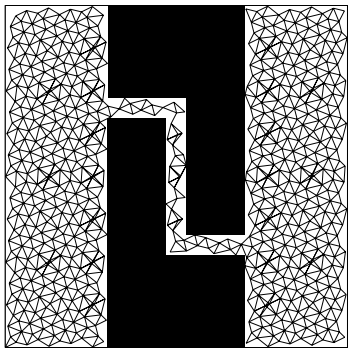
\includegraphics[width=0.35\textwidth]{images/Q-PRM.png}
        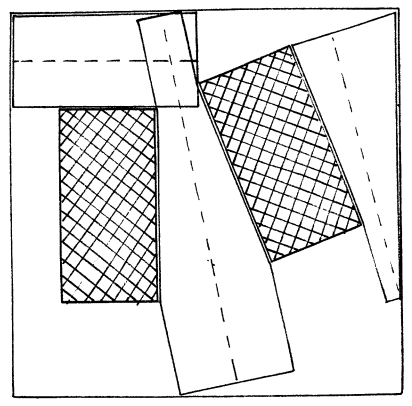
\includegraphics[width=0.35\textwidth]{images/cones.png}
        \caption{Muestreo del escenario por parte de ambos métodos}
        \label{fig:muestreo_metodos}
\end{figure}  

La mayor diferencia se encuentra en el modo de muestrear el espacio. El Q-PRM soluciona esto creando una secuencia determinista de muestras pseudo-aleatorias que conformarán un grafo a través del cual se buscará el camino mas rápido, mientras que en el caso del método de los conos generalizados se busca representar el espacio libre empleando dicha figura geométrica para luego buscar el camino. En la figura \ref{fig:muestreo_metodos} se puede observar como trabajan ambos métodos\\

Esta es una de las desventajas del algoritmo planteado por Brooks, ya que necesita representar todo el $C_free$ para encontrar una trayectoria, mientras que en el Q-PRM solo necesitas saber que los nodos y las conexiones que conforman el grafo no colisionan con ningún obstáculo. Además de esto, la complejidad de implementar el Q-PRM es bastante inferior, ya que utiliza conjuntos de muestras ya definidos en el campo de las matemáticas, por lo que todo se reduce a elegir cual de los distintos grupos se va a utilizar. En cuanto a la crítica que Yongji Wang hace al trabajo de Brooks, igualmente sería aplicable al algoritmo Q-PRM, ya que también sería necesario poder realizar movimientos de rotación pura.